\documentclass[ngerman]{dtk}
\usepackage[utf8]{inputenc}
\usepackage[T1]{fontenc}
\title{Wörter zählen in \LaTeX-Dokumenten}

\Author{Uwe}{Ziegenhagen}{Berlin}
%\address{J.E.}{Mand}{Weiter Weg 22\\99999 Hinterm Berg}

\begin{document}

\maketitle

%%-----------------------------------------------------------------------------
%% Die Definition von lokalen Makros und Umgebungen erfolgt hier.
\newcommand{\bs}{\symbol{`\\}}
\newcommand{\hint}[1]{#1}
\newcommand{\hintb}[1]{#1}


% http://folk.uio.no/einarro/Comp/texwordcount.html
% http://lwc.sourceforge.net/

% http://ubuntu.wordpress.com/2007/02/07/true-word-count-in-latex/

% http://www.google.de/search?q=latex+word+counting+wc&sourceid=navclient-ff&ie=UTF-8&rlz=1B3GGGL_deDE217DE217


\markboth{Wörter zählen}{Wörter zählen}

%%-----------------------------------------------------------------------------
\begin{abstract}
Die Information über die Anzahl der Wörter und Absätze ist in gängigen Textverarbeitungen meist nur einen Mausklick entfernt, einige \LaTeX-Editoren wie Kile bieten diese Funktion ebenso. Doch abseits von Kile \& Co ist man auf die Hilfe externer Tools angewiesen, von denen ich einige in diesem Artikel vorstellen möchte.
\end{abstract}

\section{wordcount}

Das Testdokument besteht aus 100 Worten des bekannten \hint{Lorem Ipsum} Textes, zwei \hint{section} Überschriften mit insgesamt drei Worten und drei Formeln, die jeweils ein Wort in einem \hintb{text} Befehl ausgeben, also insgesamt 106 Worte. 

Unter Unix/Linux ist \hint{wc} die Standardlösung, wenn es um das Ermitteln der Wörter eines Textes geht. \hint{wc testdokument.tex} gibt die die Anzahl der Zeilen, Wörter und Zeichen aus, im Beispiel \hint{21 130 997}. An der Ausgabe wird klar, dass \hint{wc} nicht für die explizite Verwendung mit \LaTeX~ ausgelegt ist, da alle \LaTeX-spezifischen Kommandos als Wörter gezählt werden. 

Das das Bereinigen der Quelldatei mittels \hint{untex} ist vom Ergebnis her noch schlechter, da zu wenige \LaTeX-Befehle entfernt werden. Ein \hint{untex testdokument| wc} gibt deutlich vom richtigen Ergebnis abweichende \hint{21 134 880} aus.  TeX Live bietet zusätzlich das Kommando \hint{detex}, das ebenso versucht, \LaTeX-Kommandos aus dem Dokument zu entfernen. Angewandt auf unser Dokument ergeben sich gute 108 Wörter. Dabei entfernt \hint{detex} zwar Konstrukte wie \hintb{documentclass}, \hintb{section} und \hintb{usepackage}, lässt aber die Paketnamen im Text stehen. Dafür entfernt es rigoros mathematischen Input, das \hintb{text\{Pythagoras\}} in den Formeln wird daher auch unterschlagen. 

Als Alternative zum \glqq Entrümpeln\grqq der \LaTeX-Datei kann auch die PDF-Datei per \hint{pdftotext} umgewandelt werden. Dessen Ausgabe unterdrückt naturgemäß alle LaTeX-Befehle, wandelt jedoch auch die Formeln um. Das Ergebnis von \hint{wc}, angewandt auf die Ausgabe von \hint{pdftotext}, ergibt 125 Wörter. Verwandte Resultate erbringt auch \hint{ps2ascii}, das 123 Wörter zählt.

\section{\textit{LaTeX word count} von E. R\o dland}

Sehr gute Ergebnisse erzielt \hint{LaTeX word count} von Einar Andreas R\o dland, das unter \url{http://folk.uio.no/einarro/Comp/texwordcount.html} zum Download bereitsteht und in seiner neuesten Version 2.2.beta auch mit UTF-8 und Chinesisch/Japanisch umgehen kann. Das in Perl geschriebene Programm steht online zur Verfügung und kann auch heruntergeladen werden. Die Resultate, verglichen mit den bisher vorgestellten Lösungen, sind deutlich besser: Es werden 100 Worte im Text gefunden und drei in den  Überschriften. Ignoriert werden nur die Worte, die innerhalb der \hintb{text} Umgebungen stehen.

\begin{figure}
	\centering
		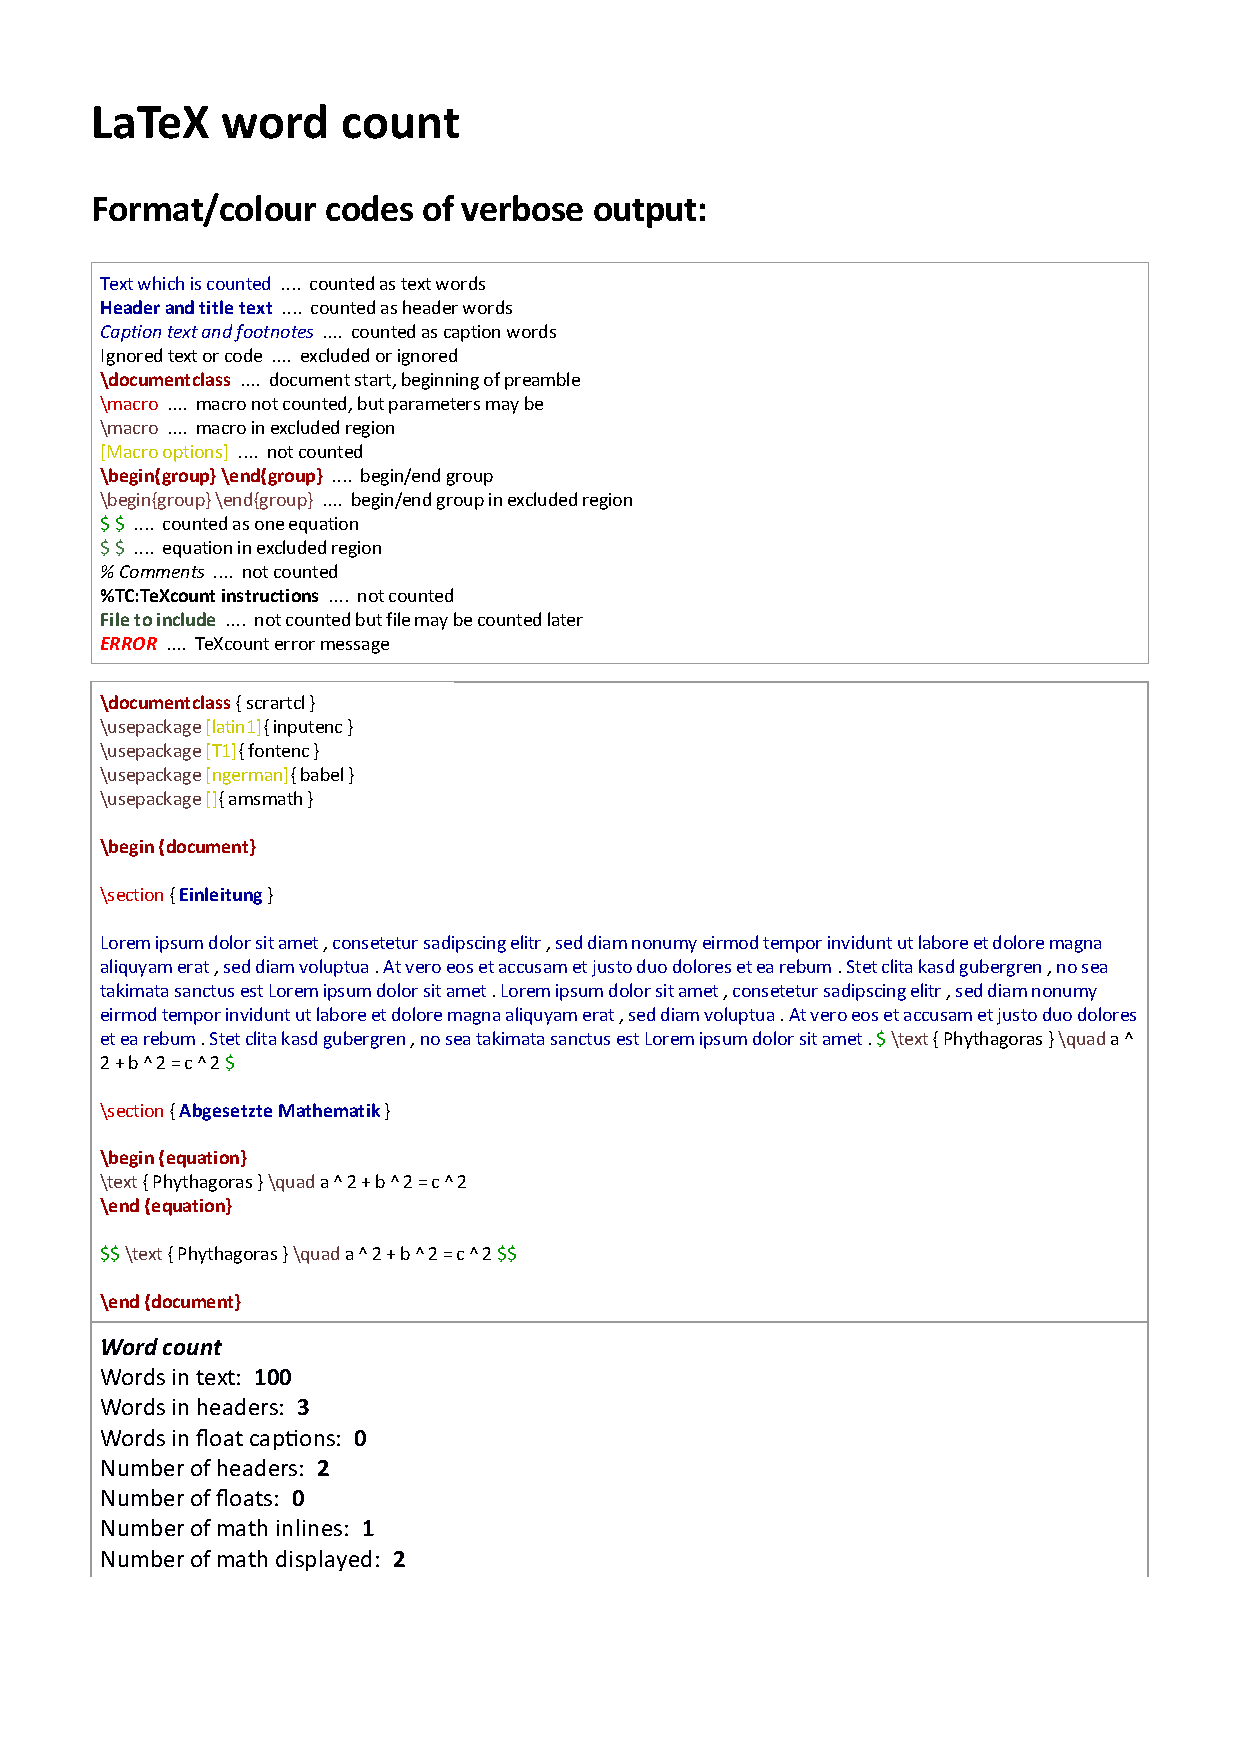
\includegraphics[width=\textwidth]{texwordcount.pdf}
		\caption{Ausgabe von \hint{LaTeX word count} für das Testdokument}
	\label{fig:texwordcount}
\end{figure}

\section{texWordCount}

Ebenfalls in Perl geschrieben ist das aus Singapur stammende \hint{texWordCount}, das unter \url{http://wing.comp.nus.edu.sg/~min/texWordCount/} zum Download und online verfügbar ist. Rein qualitativ ist es deutlich schlechter als \hint{LaTeX word count}, für das Testdokument errechnet es 122 Wörter.

\section{LaTeX Word Counter}

\hint{LaTeX Word Counter} ist ein Java-Programm und über \url{http://sourceforge.net/projects/lwc/} erhältlich. Das Programm startet eine kleine grafische Nutzeroberflöche, über die die durchzuzählende Datei geladen wird. 

\section{Zusammenfassung}

Von allen vorgestellten Lösungen gefällt \hint{LaTeX word count} am besten. Von allen Programmen kam es am nächsten an die tatsächliche Wortzahl heran und besticht durch die gut gemachte Webseite und die Tatsache, dass es vom Autor aktiv gepflegt wird. Im Einzelfall hängt es jedoch ab, welche Struktur das Dokument hat, in dem man die Wörter zählen möchte. Bei großen text-lastigen Dokumenten spielt es sicherlich eine geringere Rolle, ob Formeln bzw. der Text in Formeln gezählt werden als naturwissenschaftlichen Veröffentlichungen. 

\end{document}
